\documentclass[10pt,a4paper,english]{article}
\usepackage{babel}
\usepackage{ae}
\usepackage{aeguill}
\usepackage{shortvrb}
\usepackage[latin1]{inputenc}
\usepackage{tabularx}
\usepackage{longtable}
\setlength{\extrarowheight}{2pt}
\usepackage{amsmath}
\usepackage{graphicx}
\usepackage{color}
\usepackage{multirow}
\usepackage{ifthen}
\usepackage[DIV12]{typearea}
% generated by Docutils <http://docutils.sourceforge.net/>
\newlength{\admonitionwidth}
\setlength{\admonitionwidth}{0.9\textwidth}
\newlength{\docinfowidth}
\setlength{\docinfowidth}{0.9\textwidth}
\newlength{\locallinewidth}
\newcommand{\optionlistlabel}[1]{\bf #1 \hfill}
\newenvironment{optionlist}[1]
{\begin{list}{}
  {\setlength{\labelwidth}{#1}
   \setlength{\rightmargin}{1cm}
   \setlength{\leftmargin}{\rightmargin}
   \addtolength{\leftmargin}{\labelwidth}
   \addtolength{\leftmargin}{\labelsep}
   \renewcommand{\makelabel}{\optionlistlabel}}
}{\end{list}}
\newlength{\lineblockindentation}
\setlength{\lineblockindentation}{2.5em}
\newenvironment{lineblock}[1]
{\begin{list}{}
  {\setlength{\partopsep}{\parskip}
   \addtolength{\partopsep}{\baselineskip}
   \topsep0pt\itemsep0.15\baselineskip\parsep0pt
   \leftmargin#1}
 \raggedright}
{\end{list}}
% begin: floats for footnotes tweaking.
\setlength{\floatsep}{0.5em}
\setlength{\textfloatsep}{\fill}
\addtolength{\textfloatsep}{3em}
\renewcommand{\textfraction}{0.5}
\renewcommand{\topfraction}{0.5}
\renewcommand{\bottomfraction}{0.5}
\setcounter{totalnumber}{50}
\setcounter{topnumber}{50}
\setcounter{bottomnumber}{50}
% end floats for footnotes
% some commands, that could be overwritten in the style file.
\newcommand{\rubric}[1]{\subsection*{~\hfill {\it #1} \hfill ~}}
\newcommand{\titlereference}[1]{\textsl{#1}}
% end of "some commands"
\ifthenelse{\isundefined{\hypersetup}}{
\usepackage[colorlinks=true,linkcolor=blue,urlcolor=blue]{hyperref}
}{}
\title{RSnet2}
\author{}
\date{}
\hypersetup{
pdftitle={RSnet2}
}
\raggedbottom
\begin{document}
\maketitle

\setlength{\locallinewidth}{\linewidth}


%___________________________________________________________________________

\hypertarget{the-rsnet-network-example}{}
\pdfbookmark[0]{The RSnet network example}{the-rsnet-network-example}
\section*{The RSnet network example}
\label{the-rsnet-network-example}

RSnet is a demonstration of a simple network, consisting of a square grid
of simplified neocortical regular spiking pyramidal cells, each one coupled
with excitory synaptic connections to its four nearest neighbors.  A brief
current injection pulse to the soma of a specified cell (typically in the
center or lower left corner) starts a propagating wave of excitation.

The original GENESIS 2 script 'RSnet.g' was used as an example in the
GENESIS Modeling Tutorial section ``Creating large networks with GENESIS''
(\href{http://www.genesis-sim.org/GENESIS/UGTD/Tutorials/genprog/net-tut.html}{http://www.genesis-sim.org/GENESIS/UGTD/Tutorials/genprog/net-tut.html}).

This short tutorial describes the use of 'planarconnect' and related commands
to build a network from prototype cells, by analyzing the 'RSnet.g'
script.  It should be consulted for background on the RSnet2 scripts.

The simulation script was designed to be easily modified to allow one to
use other cell models, implement other patterns of connectivity, or to
augment with a population of inhibitory interneurons and the several other
types of connections in a cortical network.  It has since been further
extended to more biologically interesting networks with both excitatory and
inhibitory connections, such as the Vogels and Abbott (2005) model GENESIS
implementation with Hodgkin-Huxley dynamics. This was used as a benchmark
for neural simulators in the review by Brette et al. (2007).  This model
may be found at
\href{http://www.genesis-sim.org/GENESIS/UGTD/Tutorials/networks/Vogels-Abbott_net/index.html}{http://www.genesis-sim.org/GENESIS/UGTD/Tutorials/networks/Vogels-Abbott{\_}net/index.html}


%___________________________________________________________________________

\hypertarget{the-rsnet2-series-of-scripts}{}
\pdfbookmark[0]{The RSnet2 series of scripts}{the-rsnet2-series-of-scripts}
\section*{The RSnet2 series of scripts}
\label{the-rsnet2-series-of-scripts}

Although the RSnet model is too simple to be of serious scientific interest
without the extensions described above, it illustrates the same GENESIS
objects and commands that are used in much more detailed cortical models.
With no competing inhibition, the general behavior of the model can easily
be understood, and the correct behavior recognized from an analysis of the
output.

The RSnet2 scripts are reorganized and more modular versions of RSnet.g.
Unless otherwise noted, they are identical to each other, except for the
values of some flags that are used to determine which features to enable.
This allows, for example, 'RSnet2-G3.g' to run in batch mode with no
graphics, using only the most basic G2 functions needed to run the network
model and output the results with an 'asc{\_}file' object.  The other change
that was made from the original version was to replace the use of
'planarconnect' with the more general three-dimensional command
'volumeconnect', and 'planarweight' and 'planardelay' by 'volumeweight' and
'volumedelay'.

The main scripts are:

\emph{RSnet2-G2.g} - This has the definitions:
\begin{quote}{\ttfamily \raggedright \noindent
str~RUNID~=~"0000"~~~~~~~~//~default~ID~string~for~output~file~names~\\
~\\
int~graphics~=~1~//~display~control~panel,~graphs,~optionally~net~view~\\
int~batch~=~0~~~~~~~~~~~//~if~(batch)run~with~default~parameters~\\
int~netview{\_}output~=~1~~//~Record~network~output~(soma~Vm)~to~a~file~\\
int~binary{\_}file~=~1~~~~~//~if~0,~use~asc{\_}file~to~produce~ascii~output~\\
~~~~~~~~~~~~~~~~~~~~~~~~//~else~use~disk{\_}out~to~produce~binary~FMT1~file~\\
int~EPSC{\_}output~=~0~//~output~summed~EPS~currents~to~file~(not~implemented)~\\
int~connect{\_}network~=~1~~~~~~~~//~Set~to~0~for~debugging~with~unconnected~cells~\\
~\\
int~netview~=~1~//~show~network~activity~view~(slower,~but~pretty)~\\
int~hflag~=~0~~~~//~use~hsolve~if~hflag~=~1~\\
int~hsolve{\_}chanmode~=~0~//~Only~applies~if~hflag~=~1~\\
int~G3{\_}hacks~=~0~//~Special~treatment~for~things~that~G3~can't~yet~do~\\
~~~~~~~~~~~~~~~~~//~Also~needed~for~G2~with~hsolve~\\
//~At~present,~this~is~the~only~stimulus~option~\\
str~input{\_}model~=~"pulsed{\_}inject"~//~pulsed~current~injection~to~soma
}\end{quote}

RSnet2-G2.g uses the included file RSnet2-graphics.g to provide a GUI for
control of the simulation and visualization of the spreading network
activation, using the XODUS 'xview' object.  XODUS dialog boxes (labeled
textfields) on the control panel invoke script functions for setting many
of the cell, network, and injection parameters.  A different ``run ID''
string may be specified in order to save results from different runs.  All
versions of the this script create a summary file with a name of the form
'run{\_}summary{\_}{\textless}RUNID{\textgreater}.txt'.  RSnet2-G2.g records the soma Vm of each cell in
a binary file created by the 'disk{\_}out' object. The output file has a name
of the form 'Ex{\_}net{\_}Vm{\_}{\textless}RUNID{\textgreater}.dat', and can be used for post-run analysis
by the script 'replay{\_}RSnet2.g' described below.

The results of running this simulation with default parameters are
included in the directory with the scripts as 'run{\_}summary{\_}0000-def.txt'
and 'Ex{\_}net{\_}Vm{\_}0000-def.dat'.

\emph{RSnet2-h4.g} - These definitions are different from RSnet2-G2.g:
\begin{quote}{\ttfamily \raggedright \noindent
str~RUNID~=~"0000h4"~~~~~~//~default~ID~string~for~output~file~names~\\
~\\
int~netview~=~0~//~show~network~activity~view~(slower,~but~pretty)~\\
int~hflag~=~1~~~~//~use~hsolve~if~hflag~=~1~\\
int~hsolve{\_}chanmode~=~4~//~Only~applies~if~hflag~=~1~\\
int~G3{\_}hacks~=~1~//~Special~treatment~for~things~that~G3~can't~yet~do~\\
~~~~~~~~~~~~~~~//~Also~needed~for~G2~and~hsolve
}\end{quote}

This illustrates the creation of a network with cells that have been taken
over by the hsolver in chanmode 4.  Because the xview display cannot
operate with the higher chanmodes, the netview display is disabled.
'G3{\_}hacks' is used because INJECT messages from a pulsegen to a compartment
do not work in \emph{GENESIS 2} in the higher chanmodes.  This is not required
in chanmode 1, which also allows the netview.  The default simulation
produces a file 'Ex{\_}net{\_}Vm{\_}0000h4.dat', that when analyzed with
'replay{\_}RSnet2.g', produces results that are qualitatively similar,
but not exactly the same as RSnet2-G2.g.  For example, compare
the two contour plots \href{figures/freqplot-0000-def.png}{freqplot-0000-def.png} and \href{figures/freqplot-0000h4.png}{freqplot-0000h4.png}

\emph{RSnet2-G3.g} - These definitions are different from RSnet2-G2.g:
\begin{quote}{\ttfamily \raggedright \noindent
int~graphics~=~0~//~display~control~panel,~graphs,~optionally~net~view~\\
int~batch~=~1~~~~~~~~~~~//~if~(batch)run~with~default~parameters~\\
int~binary{\_}file~=~0~~~~~//~if~0,~use~asc{\_}file~to~produce~ascii~output~\\
~~~~~~~~~~~~~~~~~~~~~~//~else~use~disk{\_}out~to~produce~binary~FMT1~file~\\
int~netview~=~0~//~show~network~activity~view~(slower,~but~pretty)~\\
int~G3{\_}hacks~=~1~//~Special~treatment~for~things~that~G3~can't~yet~do~\\
~~~~~~~~~~~~~~~//~Also~needed~for~G2~and~hsolve
}\end{quote}

Here, the default simulation (RUNID = ``0000'') is run for the default
time tmax = 0.5 sec.  There are no graphics, and the output file is
a plain text file created by 'asc{\_}file' with a column for each cell
and a line for each output time step.

The use of 'G3{\_}hacks' replaces the pulsegen with a short sequence of steps
with constant injection, followed by the the remainder of the run with no
injection.  It also replaces the uses of single commands having wildcard
paths by loops over all cells, because ns-sli cannot currently use this
wildcard notation.  For example, the 'volumeweight' and 'volumedelay'
commands are replaced by with loops over all cells and all synapses, in
order to set the synapse weight and delay.

It is difficult to compare the results with those of RSnet2-G2.g because
the 'disk{\_}in' object used in 'replay{\_}RSnet2.g' cannot properly read
ascii files with more than 16 columns.  This is discussed further below.

\emph{RSnet2-STDP.g} - This has an additional flag:
\begin{quote}{\ttfamily \raggedright \noindent
use{\_}stdp~=~1~//~Use~spike~timing~dependent~plasticity~in~Ex{\_}ex~connections
}\end{quote}

and script commands to implement spike timing dependent changes in synaptic
weights.  Its use and requirements are explained in more detail below.


%___________________________________________________________________________

\hypertarget{post-run-analysis-scripts}{}
\pdfbookmark[0]{Post-run analysis scripts}{post-run-analysis-scripts}
\section*{Post-run analysis scripts}
\label{post-run-analysis-scripts}

The GENESIS 2 script 'replay{\_}RSnet2.g' is unlikely to be translated into
GENESIS 3.  It requires XODUS graphics to run, and uses a variety of
GENESIS 2 device class objects and options of the 'table' object with four
different clocks in order to collect statistics for analysis and comparison
of network behavior.  It is offered here for these reasons:
\begin{quote}{\ttfamily \raggedright \noindent
1.~At~present,~it~is~the~only~way~to~analyze~the~network~output~and~\\
~~~generate~the~files~needed~by~the~G3Plot~package.~\\
~\\
2.~It~may~be~used~as~a~prototype~for~python-based~G3~graphical~\\
~~~and~analysis~tools,~and~can~eventually~be~replaced~by~python~code.~\\
~\\
3.~It~presents~a~challenge~for~G3~implementation,~and~the~question~\\
~~~of~whether~this~sort~of~analysis~tool~should~be~scriptable~in~G3,~\\
~~~or~scripted~separately~in~python.~~The~answer~is~not~obvious.
}\end{quote}

It should be noted that the type of analysis to be performed depends
strongly on the type of network that is being modeled.  This makes it
very difficult, if not impossible, to design a general-purpose spike
analysis tool.  Some degree of scripting will be required to generate
comparable tools to 'replay{\_}RSnet2.g', whether it be with G3 objects
in a GENESIS script, or with provided python libraries of objects
that can be ``glued'' together with \emph{simple} python scripts by the user.


%___________________________________________________________________________

\hypertarget{running-replay-rsnet2-g}{}
\pdfbookmark[0]{Running replay{\_}RSnet2.g}{running-replay-rsnet2-g}
\section*{Running replay{\_}RSnet2.g}
\label{running-replay-rsnet2-g}

After starting the simulation with GENESIS 2, enter the RUNID in the top
dialog if it is other than the default ``0000'' and click ``RUN''.  As it runs
and generates the voltage plots and netview display, it will generate the
file ``spike{\_}freq{\_}{\textless}RUNID{\textgreater}.txt''.  This contains a line for each increment of
time (determined by the frequency histogram bin width) and a column for
each row in the network that gives the average firing rate of cells in that
row during that time interval.  After exiting GENESIS, the command:
\begin{quote}{\ttfamily \raggedright \noindent
rowrateplot.py~spike{\_}freq{\_}0000.txt
}\end{quote}

will generate a contour plot showing how the average frequency of cells
on each row changes with time.  The resulting plot is shown in
\href{figures/freqplot-0000-def.png}{freqplot-0000-def.png}. It shows the progressive increase in
firing rate of each row as the wave of excitation spreads.

Optionally, clicking ``Write spike times to file'' after the end of the run
will generate a file ``spike{\_}times{\_}{\textless}RUNID{\textgreater}.txt'', with the data that can be
used to generate a raster plot for the (approximately) middle cell on each
row, with the row number on the y-axis.  This may be used with:
\begin{quote}{\ttfamily \raggedright \noindent
rasterplot.py~spike{\_}times{\_}0000.txt
}\end{quote}

to produce the plot seen in \href{figures/rasterplot-0000-def.png}{rasterplot-0000-def.png}

Here, the x-axis shows the time of spike events for the (approximately)
middle cell on each row, with the row number on the y-axis.  This also
provides evidence of the expanding wave of excitation.

Clicking on ``Display Bins'' in the firing rate distribution form will
show a histogram of the firing rates of all the cells.

The ``freq{\_}form'' displays the average firing rate of cells in the network
vs. time.  It grows with time, as the propagating wave hits more cells.
The ``Row number'' dialog below the allows one to specify averages over cells
in a single row 1-32.  The default ``0'' means all rows, and should be used
when creating the output files.  The ``Bin width'' dialog is useful for
adjusting the optimum size bins for the firing frequency vs. time
calculations.  After changing one of these parameters, it is necessary
to do a RESET and RUN to generate the new data.


%___________________________________________________________________________

\hypertarget{notes-on-spike-rate-analysis}{}
\pdfbookmark[0]{Notes on spike rate analysis}{notes-on-spike-rate-analysis}
\section*{Notes on spike rate analysis}
\label{notes-on-spike-rate-analysis}

The connections in RSnet2 have a radial symmetry, connecting to nearest
neighbors, and the activation from the injected cell spreads out radially.
The script functions defined in 'replay{\_}RSnet2.g' and the included file
'analysis{\_}funcs-RSnet2.g' are based on those used to analyze a model under
development (ACnet2) of the thalamic input layer of primary auditory
cortex.  In this case, input from the thalamus is to a row of cells in
the network, and it was of interest to generate tables of the average
firing frequency of cells lying along each row at specified time intervals.
This is the analyis performed by 'replay{\_}RSnet2.g', and it makes some sense
when the the stimulated cell is a bottom row cell, because it shows the
vertical propagation of the activation.  This is the data saved to
'spike{\_}freq{\_}0000-def.txt' and is the format expected by the G3Plot
tool 'rowrateplot.py' to create the contour plot.

However, it would be better to for 'replay{\_}RSnet2.g' to group the cells by
rings around the point of injection, rather than by rows, and have a more
general version of 'rowrateplot.py'.  The latter should not be difficult,
but the GENESIS 2 (and XODUS) script programming required to make this
change in the calculation of the data to go in the spike frequency file is
large, and not worth the effort.  Other networks and groupings of cells
would require other modifications of old SLI syntax script functions.

This is the challenge for G3:

Make simple user-scriptable or GUI-configurable tools to allow one to
perform this sort of post-run analysis.  This type of analysis is not the
kind of thing that is easily done by a novice with Matlab - Matlab is more
suited to the display aspect, which can be handled by Matplotlib and other
Python tools.


%___________________________________________________________________________

\hypertarget{analyzing-asc-file-network-output}{}
\pdfbookmark[0]{Analyzing asc{\_}file network output}{analyzing-asc-file-network-output}
\section*{Analyzing asc{\_}file network output}
\label{analyzing-asc-file-network-output}

The script 'RSnet2-G3.g' creates a plain text file for the netview
output of cell membrane potentials.   The script 'replay{\_}RSnet2-asc.g'
shows how such a file can be read with 'disk{\_}in' with plain text file
format.  It runs without errors, but produces incorrect results.  This
is because the GENESIS 2 implementation of 'disk{\_}in' restricts the input file
to having no more than 16 columns per line.  As there is a column for
every cell, and 'disk{\_}in' reads a new line every time step, only the
first 16 cells of the 1024 cell network are read.  This problem should be
addressed in the G3 implementation of 'disk{\_}in'.


%___________________________________________________________________________

\hypertarget{other-files-included-here}{}
\pdfbookmark[0]{Other files included here}{other-files-included-here}
\section*{Other files included here}
\label{other-files-included-here}

\emph{RScell.p} - cell parameter file describing 'RScell' used in the network

\emph{protodefs.g} - definitions and commands to create prototype elements

\emph{DPchans.g} - functions to create the channels used in RScell

\emph{Sample output files} - from running and replaying the default 'RUNID 0000'
simulation:
\begin{quote}{\ttfamily \raggedright \noindent
run{\_}summary{\_}0000-def.txt~-~summary~file~with~most~important~parameters~\\
Ex{\_}net{\_}Vm{\_}0000-def.dat~~~-~binary~(FMT1)~file~with~network~soma~Vm~\\
spike{\_}freq{\_}0000-def.txt~~-~binned~frequency(time,~row)~for~rowrateplot.py~\\
spike{\_}times{\_}0000-def.txt~-~spike~times~of~middle~cell~on~each~row
}\end{quote}

\emph{figures/} - directory with the images saved from rowrateplot.py and
rasterplot.py


%___________________________________________________________________________

\hypertarget{notes-on-stdp}{}
\pdfbookmark[0]{Notes on STDP}{notes-on-stdp}
\section*{Notes on STDP}
\label{notes-on-stdp}

The script RSnet2-STDP.g is an illustration of an implementation of
spike timing dependent changes in the excitatory connection weights,
using the 'stdpSynchan' object instead of the 'synchan'. This requires
a recompilation of GENESIS using a patch to GENESIS 2.3.  The stdpSynchan
was developed by Jeremy Edgerton, and is available for download with
example scripts and documentation at \href{http://genesis-sim.org/libraries}{http://genesis-sim.org/libraries}.

'RSnet2-STDP.g' requires the additional files:
\begin{description}
\item[{'RScell{\_}stdp.p' - a version of RScell.p that uses stdpAMPA for the}] \leavevmode 
excitatory 'stdpSynchan' , instead of Ex{\_}channel for a 'synchan'.

\item[{'stdp{\_}functions4.g' - a variation on the 'stdp{\_}functions.g' script}] \leavevmode 
that is provided with the stdpSynchan package.  It defines functions
that are used to set up the 'stdpSynchan' tables that determine
the plasticity function to be used, and other functions for setting
up the channel.

\end{description}

At intervals during the simulation run, the script prints out the
changing weight values between cells on the left edge of the network
and those immediately above them.

A run with the default parameters produces output files for RUNID
``0000stdp''.  When these are analyzed with 'replay{\_}RSnet2.g' and the
resulting files are plotted with 'rasterplot.py' and 'rowrateplot.py',
the rasterplot, shown in \href{figures/rasterplot-0000stdp.png}{rasterplot-0000stdp.png}
shows increasing frequency of firing and then many skipped firings
on the lower rows, in comparison with \href{figures/rasterplot-0000-def.png}{rasterplot-0000-def.png}
which shows very regular firing, with no missed spikes, once the wave
hits a cell.

Likewise, the rowrateplot contour plot 'freqplot-0000stdp.png'

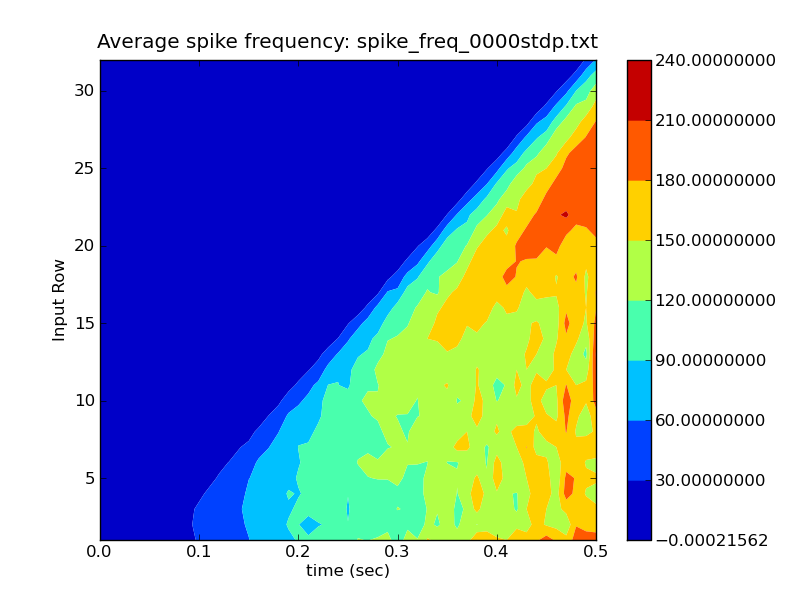
\includegraphics{figures/freqplot-0000stdp.png}

shows very irregular patches with high rates of firing, compared to
freqplot-0000-def.png.

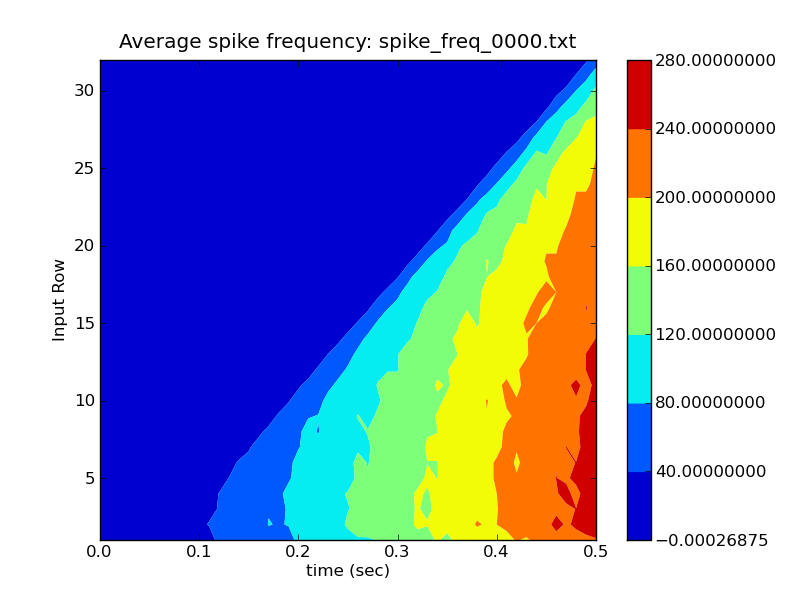
\includegraphics{figures/freqplot-0000-def.png}

This burst firing behavior can also be seen in the netview display during
the replay.


%___________________________________________________________________________

\hypertarget{figures}{}
\pdfbookmark[0]{Figures}{figures}
\section*{Figures}
\label{figures}

All figures referenced above are in the 'figures/' subdirectory.

\textbf{Note on the ReStructured Text markup used in README.txt}

The lines beginning with '..' are targets for hyperlinks to the image
files for the figures.  These will not appear in the HTML file, but:
\begin{quote}{\ttfamily \raggedright \noindent
rasterplot-0000-def.png{\_}
}\end{quote}

will show up as a hyperlink to the figure, with no trailing underscore in
the name.  The indentation used for blocks of preformatted (literal
monospaced) text that follow a double colon is necessary for identifying
the extent of the block.

The figures in the previous section that are included directly use
a target specification where they occur, e.g.:
\begin{quote}{\ttfamily \raggedright \noindent
Likewise,~the~rowrateplot~contour~plot~'freqplot-0000stdp.png'~\\
~\\
..~image::~figures/freqplot-0000stdp.png
}\end{quote}

Dave Beeman

Thu Oct 14 17:21:12 MDT 2010

\end{document}
